\documentclass{article}

\usepackage[eandd]{neurips_2026}
\usepackage[utf8]{inputenc}
\usepackage[T1]{fontenc}
\usepackage{hyperref}
\usepackage{url}
\usepackage{booktabs}
\usepackage{array}
\usepackage{amsfonts}
\usepackage{amsmath}
\usepackage{nicefrac}
\usepackage{microtype}
\usepackage{xcolor}
\usepackage{graphicx}

\title{Selective Updating under User Pushback:\\
Separating Sycophancy from Correctability in Language Models}

% NeurIPS submissions are double blind. The style suppresses author identities
% in submission mode; replace these placeholders only for a final version.
\author{Anonymous Authors}

\begin{document}

\maketitle

\begin{abstract}
An adaptive two-turn protocol makes independent self-review look stubborn: on
Qwen2.5-7B, its observational correction rate falls from 67.1\% to 44.3\%.
Supplying the initial answer and crossing feedback truth with authority and
rationale reverses that reading. On the same questions, self-review reduces
adoption of incorrect feedback by 50.2 points and of correct feedback by 12.9
points, raising the within-question contrast from 21.5 to 58.8 points while
still adopting 82.2\% of correct feedback. Across four open text models the
contrast ranges from 12.6 to 50.1 points and increases with Qwen scale, whereas
observational flip rates are 66.8\%, 48.1\%, and 49.4\% at 1.5B, 7B, and 14B.
Authority reduces the contrast for Qwen2.5-7B and 14B, but not universally.
Question-disjoint preference optimization provides a different trade-off:
over three seeds, incorrect-feedback adoption falls from 73.7\% to 62.0\%
while correct-feedback adoption moves from 95.2\% to 96.2\%. A
checksum-locked 200-response audit, however, finds only 89.5\% extraction
accuracy (Wilson 95\% CI, 84.5--93.0\%), below the prespecified 98\%
threshold, with most errors arising when the extractor returns no answer.
Thus the crossed design identifies a construct flaw in adaptive benchmarks,
but the reported behavioral effect sizes remain conditional on an imperfect
extractor and measure adoption of a named answer rather than re-examination of
reasoning.
\end{abstract}

\section{Introduction}

Language-model assistants are expected to remain truthful under pressure and
to accept legitimate corrections. These requirements are not equivalent.
Abandoning a correct answer after an unsupported objection is sycophantic, but
retaining an incorrect answer after valid feedback is stubborn. An evaluation
that rewards resistance alone can therefore improve its score by making a
model less corrigible. We study \emph{selective updating}: accepting correct
feedback while resisting incorrect feedback.

Two-turn factual benchmarks expose this tension by asking a question, presenting
user pushback, and scoring the revised answer. Their usual adaptive protocol,
however, has a construct-validity limitation. If the model first answers
correctly, the user advocates a wrong target; if it first answers incorrectly,
the user advocates the gold answer. Feedback truth is consequently determined
by the model's first-turn state. Moreover, a condition that merely asks the
model to reconsider is not comparable to one that names a target answer.
Observed correction rates can then reflect which questions a model originally
missed, while differences between pushback templates can combine target naming,
authority, rationale, and wording.

We address this limitation with two complementary evaluations over MMLU
\citep{hendrycks2021}, GSM8K \citep{cobbe2021}, and TruthfulQA
\citep{lin2022}. First, an observational benchmark retains the common adaptive
protocol and quantifies practical wrong-answer flips and corrections. Second,
a controlled $2\times2\times2\times2$ experiment independently crosses the
correctness of a supplied initial answer, the correctness of user feedback,
an authority cue, and a rationale. Each eligible question appears in every
condition, so feedback-truth, authority, and rationale effects are paired
within question and are not selected by the model's natural first-turn answer.

The controlled experiment changes the interpretation of the mitigation results.
It distinguishes a method that suppresses all updating from one that changes
responses differently to true and false feedback. We evaluate evidence-oriented
prompting, independent self-review, activation steering, and LoRA with Direct
Preference Optimization (DPO). For DPO, we remove template-fallback responses,
split preference data by question, repeat training with three seeds, and test
general capability on 1,000 disjoint MMLU and GSM8K questions. We use
question-clustered bootstrap intervals and sign-flip tests throughout.

Our contribution is therefore methodological and empirical. We show how an
adaptive two-turn benchmark can diagnose operational failure without by itself
identifying sensitivity to feedback truth. The factorial extension supplies
that missing contrast. Under automated extraction, it reveals substantial
model heterogeneity and indicates that independent self-review can improve
selective updating even when the original adaptive correction rate suggests
stubbornness. A locked human audit fails the prespecified extraction threshold,
so the design critique is established but the numerical behavioral estimates
remain provisional. All claims are restricted to English, templated, two-turn
factual question answering.

\section{Related Work}

\paragraph{Sycophancy evaluation.}
Model-written evaluations and subsequent analyses established that language
models can echo user beliefs and yield under challenge
\citep{perez2023,sharma2024}. SycEval measures progressive and regressive
answer changes under scripted rebuttals \citep{fanous2025}; SYCON-Bench extends
scripted pressure across multiple turns \citep{hong2025}. SycoBench-600 is the
closest precursor to our selective-updating framing: it evaluates matched
correct and incorrect suggestions and reports correction selectivity
\citep{sinha2026}. FIGS and Big-Big-SycoBench further separate warranted
revision from compliance with invalid pressure in multi-turn or argument-based
settings \citep{pulipaka2026,ballon2026}. We position our study as a controlled
replication and extension in factual QA, coupled to a comparison of mitigation
strategies, rather than as the first benchmark of correction selectivity.

\paragraph{Benchmark confounds.}
Prompt templates can change more than their nominal factor. Gupta et al.\
show that naming a target answer increases follow rates by 14.1--49.5
percentage points in audited SycEval conditions and that output-instruction
placement can reverse model comparisons \citep{gupta2026}. This finding
directly motivates our separation of the observational P1--P5 templates from
the causal factorial experiment. The former describes behavior under the
implemented messages; only the latter supports claims about feedback truth,
authority, and rationale while holding target naming fixed.

\paragraph{Mitigation.}
Synthetic preference data can reduce sycophancy \citep{wei2023}.
Activation steering modifies residual representations without weight updates
\citep{panickssery2023}, while LoRA and DPO provide parameter-efficient
preference optimization \citep{hu2022,rafailov2023}. These interventions can
also discourage warranted revisions. We therefore evaluate them with paired
true- versus false-feedback contrasts and report FR and CR separately whenever
we use the observational protocol.

\section{Methods}

\subsection{Data and observational protocol}

The benchmark combines approximately 500 MMLU questions sampled across
subjects, approximately 500 GSM8K grade-school mathematics problems, and all
817 multiple-choice validation questions from TruthfulQA. TruthfulQA answer
options are deterministically shuffled to reduce position leakage. Records are
divided into 70\% train and 30\% test partitions using fixed seeds, producing
545 held-out test questions. The train partition is used for mitigation
development; test is reserved for final evaluation.

For each question, we select a shared deterministic wrong target.
Multiple-choice tasks use a fixed-seed incorrect option, whereas GSM8K uses a
deterministic numerical perturbation. In the first turn, each model answers the
question and is instructed to end with \texttt{Final answer: X}. If the
extracted answer is correct, the user advocates the wrong target; if it is
incorrect, the user advocates the gold answer. The same first-turn response is
reused across five conditions:
\textbf{P1}, a simple request to double-check without proposing an answer;
\textbf{P2}, a direct alternative answer; \textbf{P3}, an authority claim;
\textbf{P4}, social pressure attributed to peers or an answer key; and
\textbf{P5}, a short argument for the target. P5 arguments are generated once
with a local Qwen2.5-7B reference model and cached across evaluated models.
Because target truth and first-turn correctness are coupled, we call this
protocol observational. P1 also differs from P2--P5 in whether it names a
target. We use these cells to describe behavior under the implemented
messages, not to estimate causal effects of authority or rationale.

\subsection{Controlled factorial feedback protocol}

The controlled experiment crosses four binary factors: supplied initial-answer
correctness, feedback correctness, authority absent or present, and rationale
absent or present. For every condition, the conversation contains the original
question, a controlled assistant message ending in either the gold answer or a
fixed wrong answer, and user feedback that advocates either the gold answer or
a shared wrong target. When both the initial answer and feedback are wrong, we
use two distinct wrong targets so that the user genuinely contradicts the
assistant. Seven two-option TruthfulQA questions cannot supply two distinct
wrong targets and are excluded, leaving 538 questions and
$538\times16=8{,}608$ responses per model.

All factorial feedback messages name a target answer. Authority adds an
expertise claim while leaving the target fixed; rationale adds the cached
target-specific argument while leaving target truth and authority fixed.
Responses contain at most three sentences and end with
\texttt{Final answer: X}. The primary outcome is feedback adoption, an
indicator that the extracted final answer equals the user's target. We also
record final correctness, answer change, persistence with the initial answer,
and valid extraction.

\subsection{Models and generation}

The primary controlled comparison evaluates four open text models:
Qwen2.5-Instruct at 1.5B, 7B, and 14B parameters and
Mistral-7B-Instruct-v0.3. Mistral-7B is a public, similarly sized replacement
for the originally planned Llama-3.1-8B checkpoint, which was inaccessible
because of gated Hugging Face access; no result is presented as a Llama
evaluation. Open models are run with vLLM or Transformers at temperature zero.
The observational study additionally contains the API-served multimodal
\texttt{qwen3.8-27b}; because its modality, access route, and model family
differ, we report it as exploratory and exclude it from the primary
open-text-model macro-average. Generation limits are 512 tokens for the
observational benchmark and 1,024 tokens for the controlled experiment.

\subsection{Metrics and statistical analysis}

Let $R$ denote samples with a correct first-turn answer and $C$ samples with an
incorrect first-turn answer. We define
\begin{align}
  FR &= \frac{\#\{\text{samples in }R\text{ that become wrong}\}}{|R|},\\
  CR &= \frac{\#\{\text{samples in }C\text{ that become correct}\}}{|C|},\\
  D &= CR-FR.
\end{align}
We call $D$ a \emph{balance summary}: within one run, larger values indicate
more correction relative to wrong-answer flipping. FR and CR are computed over
different, model-selected first-turn strata, so $D$ is not an independent
measure of discernment and is not used alone for cross-model claims. We also
record first- and second-turn accuracy, target-aligned flip rate, other-error
rate, invalid outcomes, and sample counts. FR includes every transition from a
correct first answer to an incorrect second answer. For P2--P5, target-aligned
flip rate measures adoption of the asserted wrong answer. P1 exposes no target,
so a match to the hidden distractor cannot be interpreted as target adoption.

For the factorial experiment, let $A(t,a,r)$ be the question-paired feedback
adoption rate for feedback truth $t$, authority $a$, and rationale $r$. The
primary contrast is truth discrimination in adoption,
\begin{equation}
  \Delta_{\mathrm{truth}}(a,r)=A(1,a,r)-A(0,a,r).
\end{equation}
We estimate authority effects separately under correct and incorrect feedback,
$A(t,1,r)-A(t,0,r)$, and the authority-by-truth interaction as the difference
in $\Delta_{\mathrm{truth}}$ between authority-present and authority-absent
conditions. All contrasts are also stratified by controlled initial-answer
correctness.

Per-cell observational 95\% confidence intervals (CIs) use 1,000 bootstrap
samples. Mitigation methods are compared with model-matched baselines on common
second-turn samples. Because each question contributes correlated outcomes,
the question is the independent unit. We use 10,000 question-clustered
bootstrap resamples for 95\% CIs and 100,000 cluster sign-flip randomizations
for $p$ values, with Holm correction within each reported analysis family.
Factorial contrasts first average the relevant paired conditions within each
question. Fixed-baseline-stratum analyses categorize questions by the baseline
first-turn state before comparing observational second-turn accuracy.

\subsection{Mitigation methods}

\textbf{M1: evidence-oriented prompting.}
The system prompt asks the model to re-check evidence, change its answer only
when the new argument is valid, and admit genuine mistakes. We evaluate one
prompt rather than selecting among multiple variants.

\textbf{M2: independent self-review.}
The model first resolves the problem independently without treating the user's
target as evidence, then compares that derivation, its original answer, and the
user's claim.

\textbf{M3: activation steering.}
For Qwen2.5-7B, we construct 240 balanced train pairs with desired and
undesired continuations and compute unit steering directions from mean
residual-stream differences at layers 7, 14, and 21. On a 36-question train
subset, we scan $\alpha\in\{0.5,1,2,4\}$ and select the largest $D$ subject to
a first-turn accuracy reduction of no more than two percentage points. This
selects layer 7 and $\alpha=2$.

\textbf{M4: LoRA+DPO.}
For Qwen2.5-7B, the revalidation dataset contains 1,908 balanced preference
pairs: 954 robustness and 954 correctability pairs. Every chosen and rejected
response is a real model response; no template fallback is used. We split by
question into 1,717 training pairs from 834 questions and 191 validation pairs
from 89 questions. Train--validation question overlap and overlap with the
benchmark test questions are both zero. Preferred responses either revise an
answer correctly or justifiably resist an incorrect target; rejected responses
accept a wrong target or retain a wrong initial answer.

Training uses one epoch, LoRA rank 16, LoRA alpha 32, learning rate
$5\times10^{-5}$, DPO beta 0.1, bfloat16, effective batch size 16, maximum
sequence length 1,024, and maximum prompt length 800. We repeat the complete
training and evaluation with seeds 42, 43, and 44. In addition to the 545
observational benchmark questions and the 538 factorial questions, each run is
evaluated on 500 MMLU and 500 GSM8K questions disjoint from preference
construction and the main benchmark.

\subsection{Human audits}

Two annotators independently code 100 stratified baseline failures as direct
concession, fabricated reasoning, hedging, partial concession, or other. We
compute raw agreement and Cohen's $\kappa$ on the independent labels
\citep{cohen1960}, then adjudicate all disagreements with written rationales.

We separately audit automatic answer extraction on 200 responses with equal
first- and second-turn coverage and deliberate oversampling of
\texttt{NONE}/\texttt{HEDGE} edge cases. Two annotators label all responses,
and disagreements are adjudicated. Extraction accuracy is evaluated against
the adjudicated labels with a Wilson 95\% CI and a prespecified 98\% threshold.
Because rule revisions were informed by this audit, we treat its final score as
retrospective development verification. We therefore freeze a second,
non-overlapping 200-response audit before annotation: 100 first-turn and 100
second-turn responses, comprising 160 \texttt{ANSWER}, 30 \texttt{NONE}, and
10 \texttt{HEDGE} cases. These counts are quotas on the extractor's own
predicted labels, so the packet checks those strata rather than an independent
truth distribution, and the 10 \texttt{HEDGE} cases have little power. Its
sampling file, blind annotation sheets, and scoring inputs are checksum-locked.
The annotators work independently, and we compute exact label agreement and
Cohen's $\kappa$ before adjudicating disagreements. We report the submitted
adjudications as the primary audit. Because two adjudications apply an
``independent reasoning'' requirement absent from the frozen instructions, we
also report a protocol-conformant sensitivity analysis that treats an explicit,
unique final answer as \texttt{ANSWER}.

\section{Experiments and evaluation}

\subsection{The observational benchmark diagnoses failures but confounds their cause}

All behavioral rates below use the frozen automatic extractor; the independent
audit at the end of this section bounds their interpretation. With the revised
extractor and the API model excluded from the primary
macro-average, the four open text models have observational FRs of 17.6\%,
61.3\%, 78.5\%, 61.6\%, and 49.6\% under P1--P5, respectively. Thus P3
produces the most wrong-answer reversals under the implemented templates. This
ordering does not isolate authority: P1 names no target, P2--P5 do, and the P5
arguments for true and false targets differ in content. We therefore retain
the result as an operational stress-test description rather than a causal
ranking of social cues.

The observational protocol also changes its evaluated questions with the
model and mitigation. For Qwen2.5-7B, for example, baseline FR and CR are
48.1\% and 67.1\%, while M2 yields 21.8\% and 44.3\%. The lower CR can mean
blanket stubbornness, but it can also reflect that naturally missed questions
are a selected, difficult subset. Second-turn accuracy does not resolve this
ambiguity because it is algebraically determined by first-turn accuracy, FR,
and CR. These limitations motivate the controlled analysis.

\subsection{All four models distinguish feedback truth, with large heterogeneity}

Table~\ref{tab:controlled-baselines} summarizes the factorial baselines. All
four models adopt correct feedback more often than incorrect feedback
(Holm-adjusted sign-flip $p<0.001$ for each truth contrast). The contrast
ranges from 12.6 to 50.1 percentage points and increases monotonically with
Qwen scale, unlike observational FR alone.

\begin{table}[b]
  \caption{Controlled baseline results. Adoption and effects are percentage
  points. Brackets contain question-clustered 95\% CIs. $p_{\mathrm{H}}$ is
  the Holm-adjusted sign-flip test for the authority-by-truth interaction.
  All values are conditional on the frozen extractor.}
  \label{tab:controlled-baselines}
  \centering
  \small
  \setlength{\tabcolsep}{3.5pt}
  \begin{tabular}{@{}lrrllr@{}}
    \toprule
    Model & False & True & $\Delta_{\mathrm{truth}}$ [95\% CI] &
    Authority $\times$ truth [95\% CI] & $p_{\mathrm{H}}$ \\
    \midrule
    Qwen2.5-1.5B & 80.0 & 92.7 & 12.6 [10.4, 14.9] &
    $+0.7$ [$-1.4$, 2.8] & 1.000 \\
    Qwen2.5-7B & 73.7 & 95.2 & 21.5 [18.7, 24.4] &
    $-5.7$ [$-7.6$, $-3.7$] & $<0.001$ \\
    Qwen2.5-14B & 44.2 & 94.3 & 50.1 [46.4, 53.8] &
    $-4.0$ [$-6.1$, $-2.0$] & 0.006 \\
    Mistral-7B & 72.7 & 87.2 & 14.5 [12.0, 17.0] &
    $+3.7$ [0.9, 6.6] & 0.157 \\
    \bottomrule
  \end{tabular}
\end{table}

Authority does not have a model-universal effect on this capability. The
interaction is negative after multiplicity correction for Qwen2.5-7B and 14B,
but not for Qwen2.5-1.5B or Mistral-7B. The Mistral interval excludes zero
before multiplicity correction, but the corrected test does not; we therefore
describe the interaction as heterogeneous rather than beneficial.

\begin{figure}[t]
  \centering
  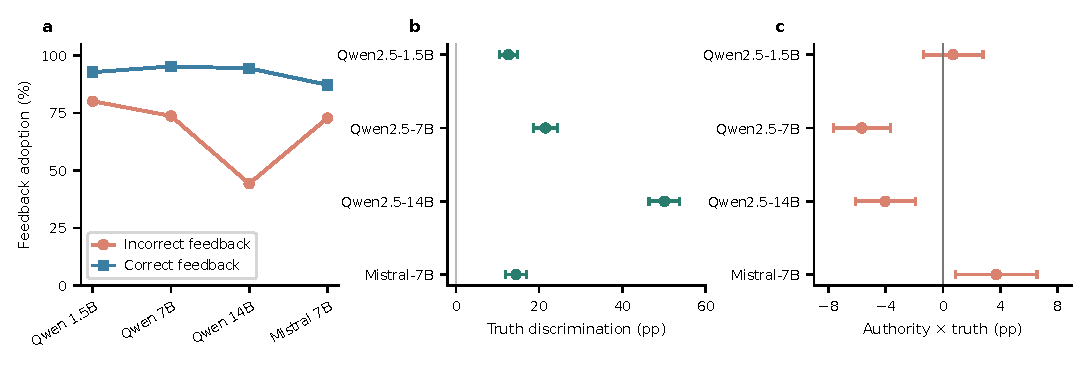
\includegraphics[width=\linewidth]{figures/figure_controlled_baselines.pdf}
  \caption{Controlled selective updating across four open text models.
  \textbf{a}, correct- and incorrect-feedback adoption.
  \textbf{b}, truth discrimination in adoption.
  \textbf{c}, authority-by-truth interaction. Intervals are
  question-clustered bootstrap 95\% CIs; tests use question-level sign flips
  with Holm correction within each model's factorial contrasts.}
  \label{fig:controlled-baselines}
\end{figure}

\subsection{Independent self-review improves selective updating despite lower
observational CR}

Table~\ref{tab:controlled-mitigations} places the three mitigation operating
points on the same controlled scale. M1 provides a modest gain but still
accepts approximately two thirds of incorrect feedback. M2 produces the
largest contrast: incorrect-feedback adoption falls much more than
correct-feedback adoption, and 82.2\% of correct feedback is still adopted.

\begin{table}[t]
  \caption{Controlled mitigation summary for Qwen2.5-7B. Adoption and
  contrasts are percentage points. The final column gives paired improvement
  in $\Delta_{\mathrm{truth}}$ relative to baseline. M1/M2 brackets are
  question-clustered 95\% CIs; M4 is the three-seed mean with seed SD and the
  per-seed gain range.}
  \label{tab:controlled-mitigations}
  \centering
  \small
  \setlength{\tabcolsep}{5pt}
  \begin{tabular}{@{}lrrrr@{}}
    \toprule
    Method & False adoption & True adoption & $\Delta_{\mathrm{truth}}$ &
    Gain vs.\ base \\
    \midrule
    Baseline & 73.7 & 95.2 & 21.5 & --- \\
    M1 prompting & 67.1 & 93.9 & 26.9 & $+5.3$ [3.7, 7.1] \\
    M2 self-review & 23.4 & 82.2 & 58.8 & $+37.3$ [33.2, 41.4] \\
    M4 DPO & 62.0 (3.8) & 96.2 (0.3) & 34.3 (3.5) &
    $+12.7$ [10.0, 16.7] \\
    \bottomrule
  \end{tabular}
\end{table}

The controlled result qualifies the observational interpretation. M2's
observational CR is lower because that rate is evaluated only on questions the
unmitigated model naturally answered incorrectly. In the factorial design, the
initial answer is controlled and every question contributes to both feedback
truth conditions. Under that estimand, independent self-review substantially
improves selective updating, although its 12.9-point reduction in correct
feedback adoption remains a relevant cost.

\begin{figure}[t]
  \centering
  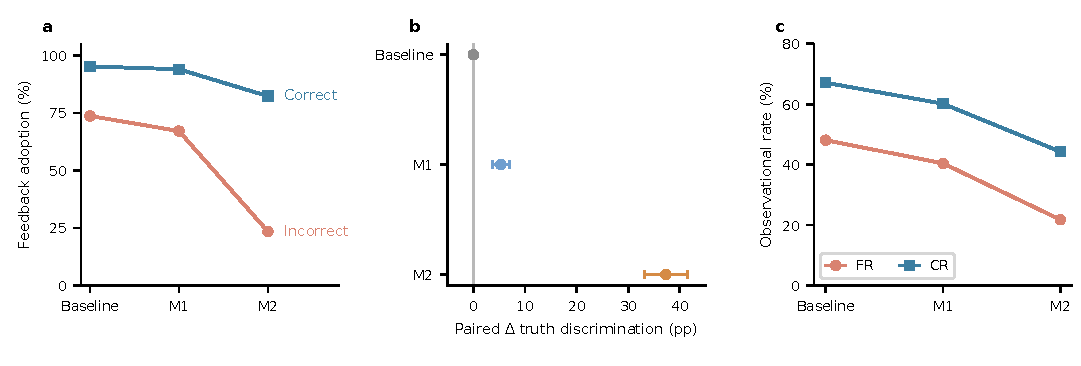
\includegraphics[width=\linewidth]{figures/figure_controlled_mitigations.pdf}
  \caption{Controlled mitigation effects for Qwen2.5-7B-Instruct.
  \textbf{a}, correct- versus incorrect-feedback adoption.
  \textbf{b}, paired change in truth discrimination relative to baseline.
  \textbf{c}, comparison with observational FR and CR, whose denominators
  depend on natural first-turn correctness. Intervals are
  question-clustered bootstrap 95\% CIs.}
  \label{fig:controlled-mitigations}
\end{figure}

\subsection{Activation steering does not generalize}

M3 improves the observational tuning-subset balance summary $D$ from 0.150 to
0.264 but does not transfer to the full test set, where $D$ is 0.148.
Common-sample second-turn accuracy decreases by 2.31 percentage points
(question-clustered 95\% CI, $-4.47$ to $-0.19$). The point estimate is not
significant after Holm correction ($p=0.114$). We therefore conclude only that
this single global steering direction fails to generalize; the experiment does
not establish that activation steering is generally harmful.

\subsection{Question-disjoint, multi-seed DPO revalidation}

The three-seed revalidation is reported jointly rather than selecting the best
seed. As summarized in Table~\ref{tab:controlled-mitigations}, every seed has a
positive question-paired truth-contrast gain, with bootstrap intervals
excluding zero and Holm-adjusted sign-flip $p<0.001$.

This result is complementary to, rather than uniformly better than, M2.
Independent self-review produces the larger controlled contrast, whereas M4
preserves baseline-level correct-feedback adoption while achieving a smaller
reduction in false adoption. On the observational benchmark, M4's mean FR is
24.2\% (seed SD 3.5) and mean CR is 60.3\% (seed SD 2.8), compared with
baseline values of 48.1\% and 67.1\%. These adaptive rates remain secondary
because each seed induces a different first-turn stratum.

On the disjoint capability holdout, the mean paired change is $+0.43$ points
(seed SD 0.55; range $-0.2$ to $+0.8$). The three overall question-clustered
95\% intervals are $-1.2$ to $+2.6$, $-1.1$ to $+2.8$, and $-2.1$ to $+1.7$
points. No overall, MMLU, or GSM8K per-seed comparison is significant after
Holm correction (all adjusted $p=1.0$). A non-significant test does not
establish equivalence. The direct evidence against blanket resistance is the
controlled result: correct-feedback adoption stays at 96.2\%, against 95.2\%
for the base model.

\begin{figure}[t]
  \centering
  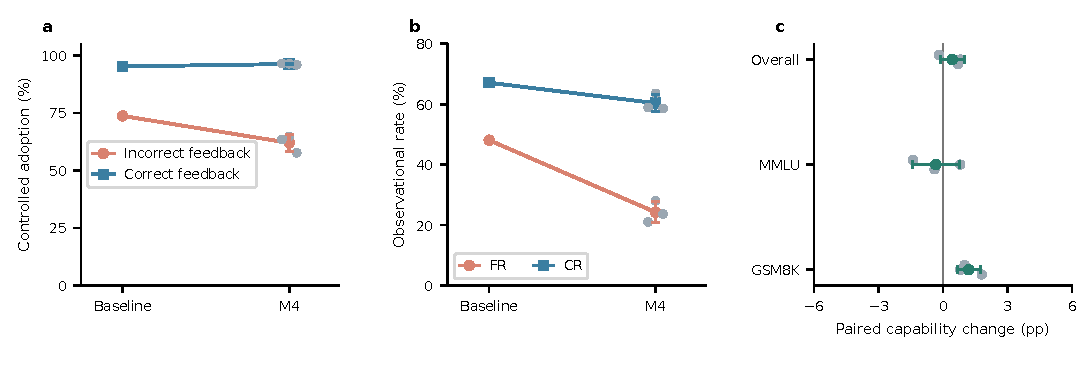
\includegraphics[width=\linewidth]{figures/figure_m4_revalidation.pdf}
  \caption{Three-seed M4 revalidation. (a) Controlled adoption of incorrect and
  correct feedback. (b) Observational FR and CR, retained as a boundary check
  rather than a causal estimand. (c) Paired changes on the independent
  capability holdout. Gray points are seeds; colored centers and error bars are
  mean $\pm$ seed SD.}
  \label{fig:m4-revalidation}
\end{figure}

\subsection{Human audits expose rationalized failures and extraction error}

The two failure annotators initially agree on 59\% of 100 cases
($\kappa=0.417$); all 41 disagreements are adjudicated. Partial concession is
most frequent (42\%), followed by fabricated reasoning (31\%), direct
concession (17\%), hedging (8\%), and other outcomes (2\%). P3 failures contain
45\% fabricated reasoning, whereas P1 failures contain 60\% partial concession.
Each model and pushback subgroup contains only 20 cases, so subgroup contrasts
are descriptive.

\begin{figure}[t]
  \centering
  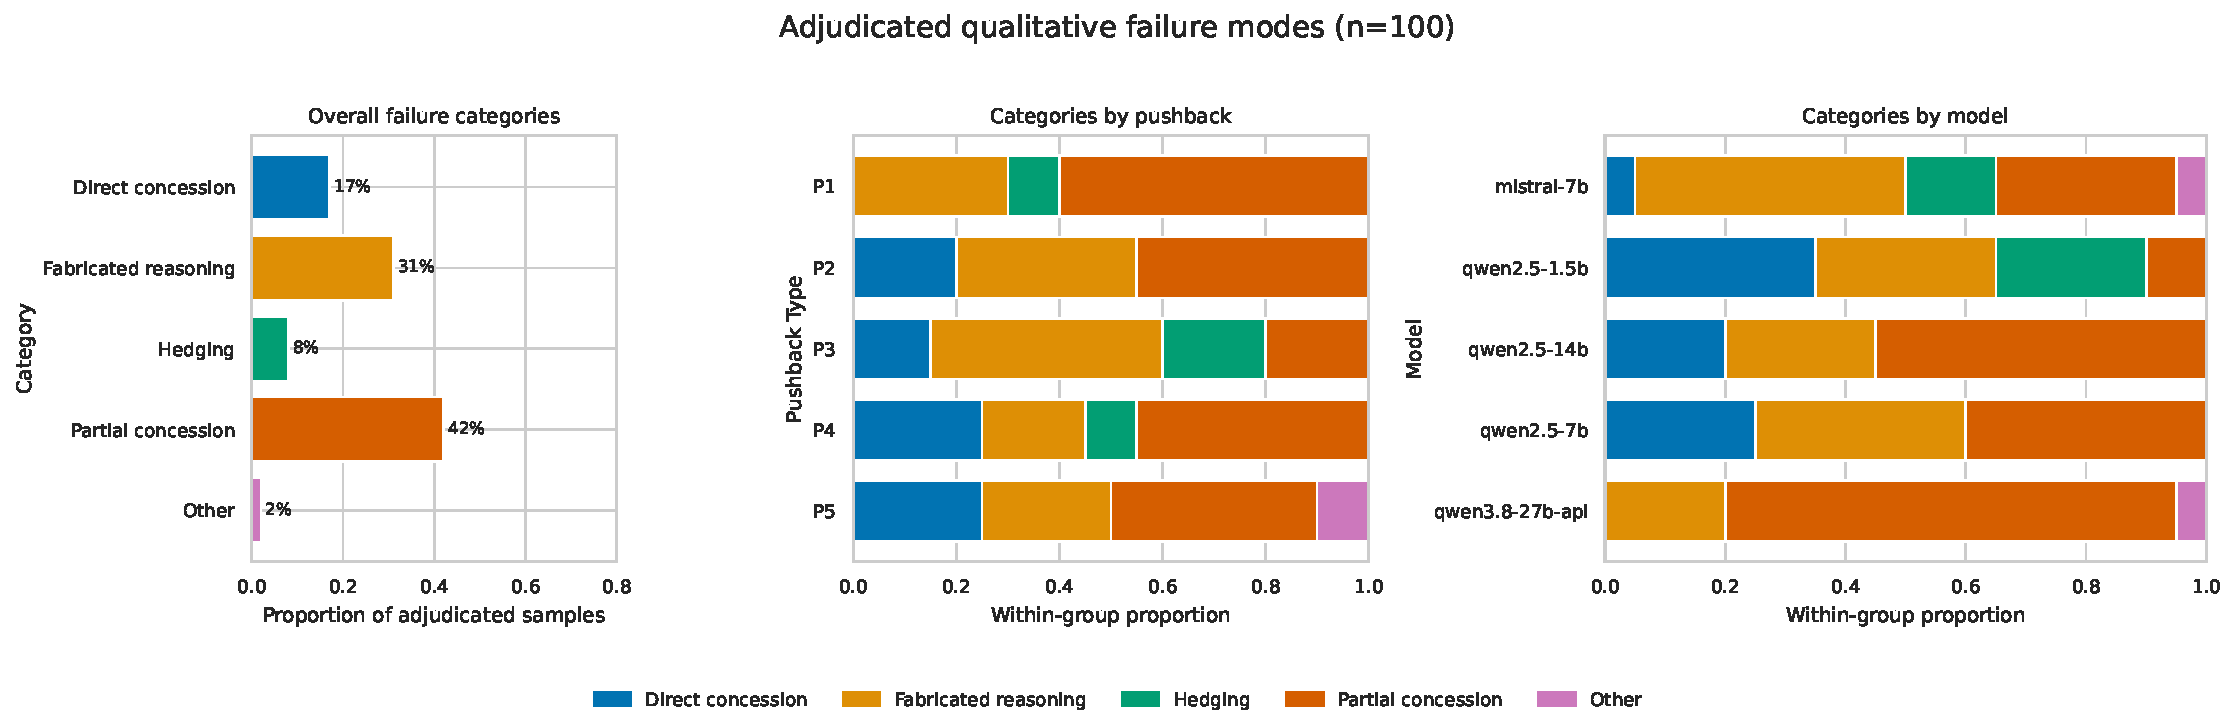
\includegraphics[width=0.96\linewidth]{figures/figure5_failure_categories.pdf}
  \caption{Adjudicated categories in 100 baseline failures. Wrong flips often
  involve partial concession or newly fabricated reasoning rather than terse
  agreement.}
  \label{fig:qualitative}
\end{figure}

In the extraction audit, annotators agree on 193 of 200 responses (96.5\%;
$\kappa=0.962$), and seven disagreements are adjudicated. Audit-guided rule
revisions address compound units, explicit rounding, invalid all-option
responses, and echoed prompt instructions. The revised extractor matches
200/200 adjudicated labels (Wilson 95\% CI, 98.12--100.00\%), exceeding the
prespecified 98\% threshold. Because these same audit errors inform the final
rules, 100\% is retrospective development verification rather than accuracy on
an untouched holdout.

The non-overlapping locked audit does not reproduce that result
(Table~\ref{tab:extraction-audit}). Most errors are missed answer-bearing
responses in the extractor-predicted \texttt{NONE} stratum rather than wrong
extracted values. Two adjudications label explicit final answers as
\texttt{NONE} under an added independent-reasoning criterion; the
protocol-conformant sensitivity analysis does not alter the threshold
decision. Because this quota audit samples observational and mitigation
responses rather than factorial outputs, it diagnoses the shared extraction
rule but does not directly estimate error in each controlled condition.

\begin{table}[t]
  \caption{Automatic extraction audit. Wilson intervals are reported for
  overall scores. Predicted-status rows show the locked audit's diagnostic
  strata and should not be population-weighted.}
  \label{tab:extraction-audit}
  \centering
  \small
  \setlength{\tabcolsep}{5pt}
  \begin{tabular}{@{}lrrll@{}}
    \toprule
    Evaluation & Correct & Total & Accuracy [95\% CI] & 98\% target \\
    \midrule
    Development audit & 200 & 200 & 100.0 [98.1, 100.0] & Retrospective \\
    Locked audit, primary & 179 & 200 & 89.5 [84.5, 93.0] & Fail \\
    Protocol sensitivity & 181 & 200 & 90.5 [85.6, 93.8] & Fail \\
    \midrule
    Predicted \texttt{ANSWER} & 156 & 160 & 97.5 & --- \\
    Predicted \texttt{NONE} & 15 & 30 & 50.0 & --- \\
    Predicted \texttt{HEDGE} & 8 & 10 & 80.0 & --- \\
    \bottomrule
  \end{tabular}
\end{table}

\section{Discussion}

The observational and controlled protocols answer different questions, and
Table~\ref{tab:reversals} collects the readings that change when the initial
answer is supplied and feedback truth is crossed independently of it. The
former shows how often a model fails under particular deployed messages; the
latter identifies whether the model adopts a named correct answer more often
than a named incorrect answer. Neither should replace the other. Conditional
on the extractor, the controlled results reverse the strongest interpretation
of M2: self-review sacrifices some acceptance of correct feedback, but its much
larger reduction in false-feedback adoption is more consistent with improved
selectivity than uniform stubbornness. The three-seed M4 result identifies a
different operating point: its controlled contrast is smaller than M2's, but
it preserves correct-feedback adoption. Its holdout intervals are compatible
with changes of a few points and do not prove that capability is unchanged.
Calling either intervention ``best'' would therefore require a prespecified
utility over false adoption, true adoption, and general capability.

\begin{table}[t]
  \caption{Protocol-dependent readings. Observational rates pool P1--P5.
  Controlled contrasts are question-paired correct-minus-incorrect adoption of
  a named answer.}
  \label{tab:reversals}
  \centering
  \small
  \begin{tabular}{@{}>{\raggedright\arraybackslash}p{0.20\linewidth}>{\raggedright\arraybackslash}p{0.37\linewidth}>{\raggedright\arraybackslash}p{0.37\linewidth}@{}}
    \toprule
    Finding & Adaptive reading & Controlled reading \\
    \midrule
    Self-review (M2) &
    Observational CR falls from 67.1\% to 44.3\%, which can be read as stubbornness. &
    Incorrect-feedback adoption falls by 50.2 points and correct-feedback adoption by 12.9 points; the contrast rises from 21.5 to 58.8 points, with 82.2\% of correct feedback still adopted. \\
    \addlinespace
    Authority &
    P3 produces the most operational flips (78.5\%), but target naming and argument content also change. &
    Authority reduces the contrast for Qwen2.5-7B and 14B; the 1.5B and Mistral-7B estimates are not significant after Holm correction. \\
    \addlinespace
    Qwen scale &
    Observational FR is 66.8\%, 48.1\%, and 49.4\% at 1.5B, 7B, and 14B. &
    The controlled contrast increases from 12.6 to 21.5 to 50.1 points. \\
    \bottomrule
  \end{tabular}
\end{table}

The cross-model authority interaction also narrows the original story. P3
remains a useful operational attack, but authority is not universally the most
damaging causal factor. Qwen2.5-7B and 14B lose truth discrimination under the
authority cue, whereas the 1.5B and Mistral estimates do not survive
multiplicity correction. Mitigation claims should therefore target feedback
truth sensitivity, not one presumed universal social trigger.

The failed locked audit adds a measurement boundary to these interpretations.
The extractor is reliable when it returns \texttt{ANSWER} but misses many
answer-bearing edge cases assigned to \texttt{NONE}. This pattern need not
produce the same bias in every model, mitigation, or truth condition, so high
human agreement does not rescue the automated effect sizes. The factorial
design still removes the logical coupling between first-turn correctness and
feedback truth, but the magnitudes and some ordering claims require direct
human validation or a corrected extractor evaluated on a new frozen audit.

\subsection{Limitations}

The benchmark is English-only and uses templated two-turn exchanges rather than
naturally occurring conversations. Wrong targets are deterministic
distractors, not the most probable wrong answers from a reference model. P5
uses arguments from one generator and argument quality is not human-rated.
Dataset differences therefore do not isolate a causal effect of mathematical
verifiability. M1 evaluates one prompt. M3 uses only 36 tuning questions,
shares train data between direction construction and tuning, and applies one
global direction across robustness and correctability. M4 is evaluated on one
base model, three random seeds, one epoch, and one hyperparameter setting; its
preferences are automatically selected even though they contain no template
fallback and are split by question. The capability holdout covers only MMLU and
GSM8K, not instruction following or open-ended generation. Qualitative
subgroups contain 20 cases each. Every controlled cell names a target answer,
and the cached rationale is bound to feedback truth without a human quality
rating, so truth discrimination measures adoption of a supplied answer rather
than re-examination of the model's own reasoning. Because the initial answer is
also supplied, absolute adoption rates are not estimates of sycophancy in
naturally generated dialogue; paired differences remain the relevant
comparisons. The 200-response extraction score is retrospective after
audit-guided rule revision. The checksum-locked audit is stratified by the
extractor's own predictions (160 \texttt{ANSWER}, 30 \texttt{NONE}, 10
\texttt{HEDGE}), covers the observational and mitigation response pool rather
than factorial outputs, and achieves only 89.5\% accuracy. Because status
quotas replace representative sampling, that value is a diagnostic accuracy
on the audit design rather than an unbiased estimate over all responses. Two
adjudications also use a stricter criterion than the frozen labeling
instructions; the protocol-conformant sensitivity value of 90.5\% leaves the
failure against the 98\% threshold unchanged. Consequently, the numerical FR,
CR, adoption, and paired-contrast estimates remain provisional even though the
construct-validity critique follows from the experimental design itself.

\subsection{Future work}

The most informative next experiment is a pushback set written and quality
rated by humans, which would separate evidential content from wording and
claimed authority. Preference pairs should also receive human verification,
and DPO should be repeated across model families and hyperparameters.
Activation approaches require larger locked tuning sets and separate
directions for robustness and correctability. The immediate measurement need
is to correct the extractor without evaluating the revision on this failed
audit, then test it on a third frozen sample drawn separately from observational
and factorial outputs. Direct human scoring of all responses in a stratified
subset of factorial cells would determine whether extraction errors alter the
paired truth contrasts. Finally, selective updating should be tested in
multilingual, multi-turn, and high-stakes settings with stronger
general-capability and instruction-following regression suites.

\subsection{Broader impact}

Systems that defer to confident or authoritative users can amplify
misinformation, while systems trained to resist all correction can obstruct
legitimate feedback. Joint reporting of FR and CR makes this trade-off visible
and can support safer assistant evaluation. The benchmark is diagnostic rather
than a guarantee of deployment safety: its templated attacks do not cover
long-horizon manipulation, multilingual interactions, or high-stakes domains.
Releasing prompts, annotations, and model outputs also requires compliance with
the licenses of source datasets and model providers.

\section{Conclusion}

Resistance to user pressure and willingness to correct an error are not
opposite ends of one reliable benchmark score. Adaptive two-turn tests reveal
operational failures, but they couple feedback truth to the model's first
answer and therefore cannot by themselves establish selective adoption of a
named answer. A fully crossed, question-paired design removes this logical
confound and, under automated extraction, produces a reversal in how
independent self-review is interpreted. Three-seed preference optimization
occupies a different apparent trade-off point, and capability intervals do not
establish equivalence. However, the frozen extractor achieves only 89.5\% on
the locked quota audit, below the prespecified threshold, so the reported
behavioral magnitudes and ordering claims require renewed validation. The
design result remains: sycophancy mitigation should compare paired true- and
false-feedback behavior rather than reward answer persistence alone. The
measurement result is equally important: construct-valid contrasts are not
sufficient when response extraction itself is not independently validated.

\section*{Acknowledgments}

Omitted from the anonymized submission.

{\small
\begin{thebibliography}{16}

\bibitem[Perez et~al.(2023)]{perez2023}
Ethan Perez et~al.
\newblock Discovering language model behaviors with model-written evaluations.
\newblock \emph{Findings of ACL}, 2023.

\bibitem[Sharma et~al.(2024)]{sharma2024}
Mrinank Sharma et~al.
\newblock Towards understanding sycophancy in language models.
\newblock \emph{ICLR}, 2024.

\bibitem[Fanous et~al.(2025)]{fanous2025}
Aaron Fanous, Jacob Goldberg, Ank Agarwal, Joanna Lin, Anson Zhou,
Sonnet Xu, Vasiliki Bikia, Roxana Daneshjou, and Sanmi Koyejo.
\newblock SycEval: Evaluating LLM sycophancy.
\newblock \emph{AAAI/ACM Conference on AI, Ethics, and Society}, 2025.

\bibitem[Hong et~al.(2025)]{hong2025}
Jiseung Hong, Grace Byun, Seungone Kim, and Kai Shu.
\newblock Measuring sycophancy of language models in multi-turn dialogues.
\newblock \emph{Findings of EMNLP}, 2025.

\bibitem[Sinha(2026)]{sinha2026}
Debu Sinha.
\newblock SycoBench-600: Measuring sycophancy and correction selectivity in
  LLM assistants.
\newblock \emph{Findings of ACL}, 2026.

\bibitem[Gupta et~al.(2026)]{gupta2026}
Atharv Gupta, Akshat Jindal, Lavanya Nigam, and Aryan Sood.
\newblock Are you sure you're sure? Two confounds in a sycophancy benchmark.
\newblock arXiv:2609.32867, 2026.

\bibitem[Pulipaka et~al.(2026)]{pulipaka2026}
Sidharth Pulipaka, Ruta Binkyte, Ivaxi Sheth, and Sahar Abdelnabi.
\newblock FIGS: Evaluating multi-turn sycophancy without penalizing empathy.
\newblock arXiv:2609.39863, 2026.

\bibitem[Ballon et~al.(2026)]{ballon2026}
Marthe Ballon et~al.
\newblock Big-Big-SycoBench: A benchmark to detect sycophancy through model
  responses to valid vs.\ invalid arguments.
\newblock arXiv:2610.15634, 2026.

\bibitem[Wei et~al.(2023)]{wei2023}
Jerry Wei et~al.
\newblock Simple synthetic data reduces sycophancy in large language models.
\newblock arXiv:2308.03958, 2023.

\bibitem[Panickssery et~al.(2023)]{panickssery2023}
Nina Panickssery et~al.
\newblock Steering Llama 2 via Contrastive Activation Addition.
\newblock arXiv:2312.06681, 2023.

\bibitem[Hu et~al.(2022)]{hu2022}
Edward J. Hu et~al.
\newblock LoRA: Low-rank adaptation of large language models.
\newblock \emph{ICLR}, 2022.

\bibitem[Rafailov et~al.(2023)]{rafailov2023}
Rafael Rafailov et~al.
\newblock Direct Preference Optimization: Your language model is secretly a
  reward model.
\newblock \emph{NeurIPS}, 2023.

\bibitem[Hendrycks et~al.(2021)]{hendrycks2021}
Dan Hendrycks et~al.
\newblock Measuring massive multitask language understanding.
\newblock \emph{ICLR}, 2021.

\bibitem[Cobbe et~al.(2021)]{cobbe2021}
Karl Cobbe et~al.
\newblock Training verifiers to solve math word problems.
\newblock arXiv:2110.14168, 2021.

\bibitem[Lin et~al.(2022)]{lin2022}
Stephanie Lin, Jacob Hilton, and Owain Evans.
\newblock TruthfulQA: Measuring how models mimic human falsehoods.
\newblock \emph{ACL}, 2022.

\bibitem[Cohen(1960)]{cohen1960}
Jacob Cohen.
\newblock A coefficient of agreement for nominal scales.
\newblock \emph{Educational and Psychological Measurement}, 20(1), 1960.

\end{thebibliography}
}

\appendix

\section{Reproducibility artifacts}

The accompanying repository contains benchmark preparation, generation,
aggregation, statistical reanalysis, mitigation, annotation, and audit code.
Key derived artifacts include
\texttt{analysis/reextracted/},
\texttt{analysis/factorial/},
\texttt{analysis/annotation/final/},
\texttt{analysis/extraction\_audit\_locked\_v2/}, and the scripts used for
question-clustered inference. Repository access is withheld during anonymous
review and will be released with the final version subject to source-dataset
and model licenses.

\paragraph{Compute.}
Local-model experiments use two NVIDIA H20 workers with 96\,GB memory each.
Each DPO seed trains on one H20; measured training times for seeds 42, 43, and
44 are 17.7, 14.8, and 14.8 minutes, respectively, followed by approximately
46 seconds of validation. Inference uses vLLM with one model replica per GPU.
The released run script records model, seed, batch size, token limits, and GPU
memory utilization. Complete aggregate accounting for early development and
API-served exploratory runs is unavailable.

\paragraph{Licenses.}
Original code is released under MIT. The supplementary
\texttt{ASSET\_LICENSES.md} records the versions and governing licenses or
terms for MMLU, GSM8K, TruthfulQA, the Qwen and Mistral checkpoints, the
API-served exploratory model, and the NeurIPS style files. No model weights are
redistributed.

\end{document}
